\documentclass[leqno,10pt]{article}
\usepackage{algorithm}
\usepackage[noend]{algpseudocode}
\usepackage{hyperref}
\usepackage{float}
\def\Z{\mathbb Z}
\def\Q{\mathbb{Q}}
\def\A{\mathbb{A}}

\makeatletter
\renewcommand{\ALG@name}{Algorytm}
\makeatother

\usepackage{amsmath}
\usepackage{float}
\usepackage{delta}
\usepackage{todonotes}
\usepackage{authblk}

\newcommand{\edge}{\mbox{\rotatebox[origin=c]{90}{\ddagger}}\xspace} 

\def\marg#1{\marginpar{\scriptsize\raggedright#1}}

\begin{document}

\wtyt{Trudność w modelu zawijania białek}


\waut{Marcin Wierzbiński$^{1,2}$, Karolina L. Tkaczuk$^{2}$, Alessandro Crimi$^{2}$}


\marg{[1] Student w Wydział Matematyki, Informatyki i Mechaniki, Uniwersytet Warszawski, [2] Sano Centrum Medycyny Obliczeniowej w Krakowie}

Modelowanie wielu problemów biologicznych za pomocą matematyki, czy informatyki to bardzo ciekawy dział. W samym modelowaniu naukowcy jak zwykle chcą pokonać wyzwania, które przed nimi stoją. Jednym z takich wyzwań jest rozwiązanie deterministyczne (wielomianowe), tzw. model fałdowania hydrofobowo-polarnego białka. Okazuje się, że ten model ma bardzo dużo wspólnego z informatyką teoretyczną, a sam problem jest trudny do rozwiązania. 

W tym artykule opiszemy bardzo prosty model zawijania białka i jego interpretacje w informatyczce teoretycznej. 

\mtyt{Wstęp}
Cząsteczka białka jest tworzona przez ciąg małych cegiełek, znanych jako aminokwasy, które ostatecznie są w stanie znaleźć się w natywnym kształcie białka. Aminokwasy są małymi cząsteczkami, które są składane razem w określony sposób, aby stworzyć białka. Wyróżniamy dwadzieścia aminokwasów, a ich połączenia tworzą białka, które zwijają się w określoną funkcjonalną strukturę przestrzenną, złożoną z tzw. $\alpha$-heliks, $\beta-$-wstążek oraz pętli. Te podstawowe struktury w połączeniu ze sobą tworzą bardziej złożone przestrzennie elementy, jak na przykład $\beta-$kartka uformowana z kilku $\beta$-wstążek czy tzw. "szpilka do włosów" (ang. hairpin loop), która składa się z antyrównoległej struktury $\beta$ podtrzymywanej przez pojedynczy łańcuch polipeptydowy.  Możemy myśleć o tym jako o różnych koralikach, które łączą się ze sobą jak koraliki na sznurku, tworząc długie łańcuchy, które nazywamy polipeptydami, a te są budulcem białek. A naprawdę fajną rzeczą w aminokwasach jest to, że kiedy są ze sobą połączone, składają się, aby nadać ostateczny kształt białku. I to właśnie kształt białka tak naprawdę dyktuje, co może ono robić w komórce.

Istnieje wiele możliwości odtworzenia kształtu białka występującego w naturze. Jako tzw. złoty standard używa się krystalografii, która jest metodą eksperymentalną odtwarzania kształtu przestrzennego biała, jest to metoda bardzo czasochłonna i czasem nieskuteczna, bo nie można uchwycić kształtu białka gdyż może się ono okazać bardzo wrażliwe na czynniki zewnętrzne i niestabilne w laboratorium, co znaczy, że rozpadnie się na kawałki zanim zdążymy odtworzyć ich kształt. Dlatego zaprzęgnięto metody obliczeniowe do modelowania komputerowego struktur 3D białek. Podstawą takiego modelowania teoretycznego są istniejące już (wcześniej eksperymentalnie odtworzone za pomocą krystalografii struktury białek zebrane w bazie białek PDB www.rcsb.org). Wraz ze wzrostem naszych możliwości obliczeniowych i coraz to nowszych dostępnych metod tworzone są nowe metody odtwarzania struktur 3D. 
Duże zainteresowanie mediów w ostatnich latach zyskał projekt AlphaFold (\href{https://alphafold.ebi.ac.uk}{alphafold.ebi.ac.uk}), w którym użyta została sztuczna inteligencja do przewidywania struktur białek.

\mtyt{Model hydrofobowy-polarny(HP)}
Dzisiejsze techniki modelowania zawijania białek obejmują składanie białek, które w rezultacie dostarczają niezwykle uproszczoną wersje różnych kombinacji aminokwasów. W modelu hydrofobowo-polarnym dwadzieścia aminokwasów jest reprezentowanych jako dwa typy $H$ (aminokwas hydrofobowy) lub $P$ (aminokwas hydrofilowy). Model ten polega na osadzeniu danej skończonej sekwencji typów $s \in\{H, P\}^{k}$ o długości $k$ w danej nieskończonej kracie $\mathbb{Z}^{3}$ lub $\mathbb{Z}^2$. 
\marg{Na płaszczyźnie euklidesowej $\mathbb{R}^{3}$ zbiór $\mathbb{Z}^{3} = \{(x, y, z)| \text{ gdzie } x, y, z \in \mathbb{Z}\}$  nazywamy kratą, a jego elementy punktami kratowymi.} 

Konformacją nazwiemy przekształcenie różnowartościowe $\omega:[1 \ldots  n] \rightarrow \mathbb{Z}^{3}$ i dodatkowo dla sąsiadujących liczb naturalnych przyporządkowujemy sąsiadujące punkty z kraty tj. \marg{W matematyce często mówi się o takim przekształceniu włożenie, jest ono różnowartościowe i zachowuje wskazane własności.}
\begin{equation}
     1 \leq i<j \leq n: \omega(i) \neq \omega(j)
\end{equation}
Celem rozwiązania problemu składania białek jest znalezienie takiej konformacji sekwencji białek na siatce, aby energia całkowita $E_{c}(s , \omega)$ była zminimalizowana, dla pewnej rozsądnej definicji energii zależnej od włożenia w kratę i sekwencji typów aminokwasów. W naszym przypadku uproszczamy tę definicje:
\begin{equation}\label{basic:eng}
    \mathrm{E_{c}}(s, \omega)=\sum_{1 \leq i<j \leq n} E_{(s_{i}, s_{j})} \Delta(\omega(i), \omega(j)),
\end{equation}
Stosując wartość równą karę energetyczną $-1$ dla sąsiednich wiązań $H \edge H$: 
\begin{equation}
    E_{(s_{i}, s_{j})} = \begin{cases}
        -1 & s_{i}=H \text{ i } s_{j}=H \\ 
        0 & \text{w przeciwnym przypadku} 
    \end{cases}   
\end{equation}

I odpowiednią funkcją kodująca liczenie energii dla punktów ze sobą sąsiadujących:
\begin{equation}
    \Delta(\omega(i), \omega(j)) = 
    \begin{cases}
        0 & $\omega(i)$ \text{ i } $\omega(j)$ \text{ są sąsiadami w kracie} \\
        1 &  \text{w przeciwnym przypadku}
    \end{cases}
\end{equation}
Warto zauważyć, że energia całkowita skręcenia jest negacją liczby wiązań $H \edge H$. W tradycyjnym modelu pary $H$-ów z sekwencji $s$ nie są liczone jako formująca wiązanie. Dla uproszczenia, możemy dodać pary $H$-ów w liczeniu energii. Konwencja nie zależy w żaden sposób nie wpływa przy ustalonej sekwencji na minimalizacje energii. 
 \marg{Czyli takie punktu sąsiadujące, pomiędzy którymi nie ma trasy, pomimo tego są tam dwa H'sy.}


\begin{figure}[!htbp]
    \centering
    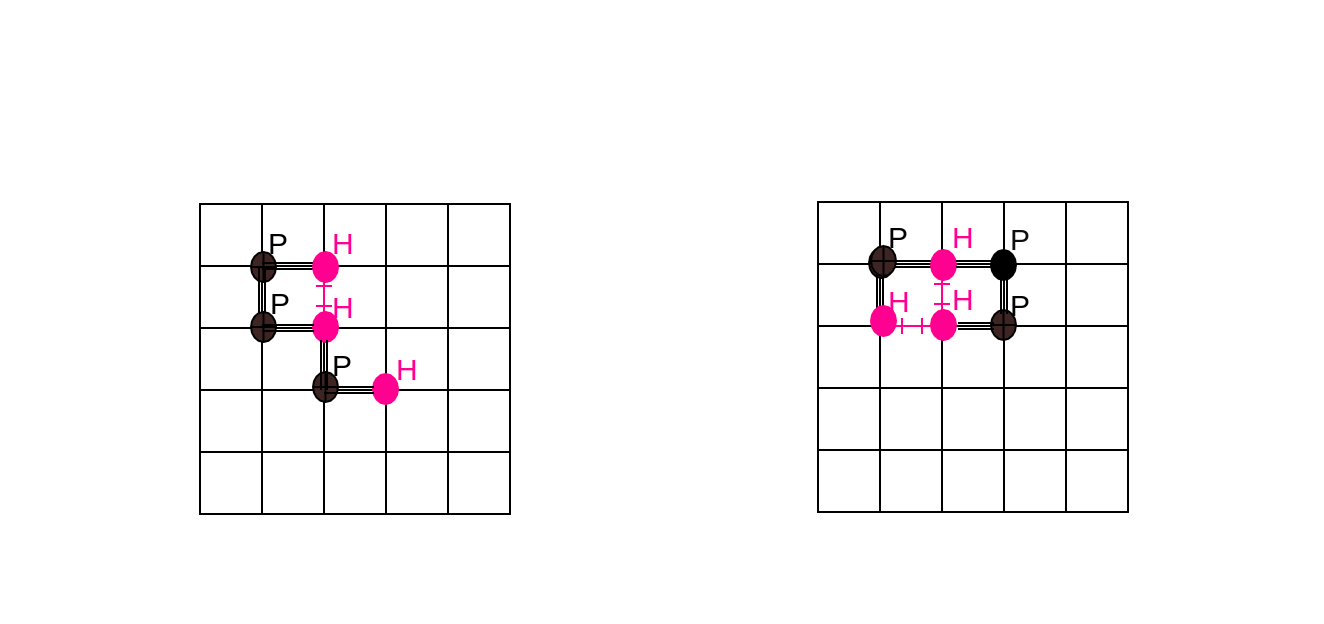
\includegraphics[width=0.9\textwidth]{diagram.png}
    \caption{Przykład konformacji dla sekwencji $s={HPPHPH}$ w kracie $\mathbb{Z}^{2}$. Po lewej stronie energia całkowita jest równa $-1$, a po prawej stronie energia całkowita jest równa $-2$. Co więcej okazuje się, że jest to optymalne globalne rozwiązanie. }
\end{figure}


\textbf{Algorytm losujący}

Jeden z pomysłów, który się nasuwa to myślenie o konformacji jako o trasie losowego spaceru długości $n$ wzdłuż siatki $\mathbb{Z}^{3}$ z ważną własności: spacer nie przecinał swojego dawnego toru, ani nie wraca z punktu z którego właśnie wyszedł. Każdemu punktowi przypisujemy literkę z sekwencji $s$. Po angielsku taka droga nazywa się \textit{Self Avoiding Walk}, w skrócie SAW. Losowanie takich spacerów to generowanie konformacji. W ten sposób można obliczać energię dla konformacji. Jednak nie mamy pewności, że algorytm losujący znajdzie minimum energii. Co więcej dla przypadku kraty $\mathbb{Z}^3$ okazuje się, że spacerując losowo mamy za dużo wyboru w każdym kroku i jest bardzo trudno zawinąć sekwencje, tak aby uzyskać globalne minimum. 


Samą liczbę konformacji potrafimy oszacować, bez dokładnej liczby. Jest to kombinatorycznie nie możliwe, chyba że dla małych przypadków $k=\{1,2\}$. Możliwym sposobem oszacowania jest metoda wzrostu zaproponowana przez Ariannę i Marshalla Rosenbluthów. Więcej w artykule z \textit{Delty} $\Delta_{15}^{6}$. Dla małych $n \in \{1,2,3\}$ można policzyć takie konformacje za pomocą kartki i ołówka. Dla większych wymiarów staje się to niemożliwe. 
\begin{table}[!htbp]
    \centering
    \begin{tabular}{c|c}
      długość sekwencji $k$   &  oszacowanie liczby konformacji \\
       1  & 6 \\
       2  & 30 \\ 
       3  & 150 \\
       4  & 725.4 \\
       5  & 3523.5 \\
       10 & 8863991.25 \\
       15 & 21283727718.75 \\
       20 & 52044761767968.75 \\
    \end{tabular}
    \caption{Oszacowanie liczby konformacji dla kraty $\mathbb{Z}^3$}
\end{table} 
\marg{Więcej jak estymować ilość takich tras jest w artykule z delty ($\Delta_{15}^{5}$): \href{http://www.deltami.edu.pl/temat/matematyka/zastosowania/2015/04/19/Monte_Carlo_spacery_i_polimery/}{Monte Carlo, Spacery I Polimery prof. Niemiro}}  
Zauważmy, że liczba takich konformacji dla liczby $k>10$ znacząco rośnie. To pokazuje, że problem już dla stosunkowo małych $k$ staje się 


\mtyt{Trudność tego modelu}
W informatyce teoretycznej wiele problemów wyraża w postaci problemów decyzyjnych. Jednak wyżej sformułowany problemem jest problemem obliczeniowym - szukamy minimum funkcji energii zadanej tak jak w równaniu \ref{basic:eng}. Zastanowimy się, czy potrafimy przeformułować to w problem decyzyjny i później w problem obliczeniowy. Podajmy jego ścisłe sformułowanie.


\textbf{Problem zawinięcia sekwencji} 
\newline
Na początku formujemy wejście tak jak w klasycznym algorytmie. 
\newline Wejście: Ustalona sekwencja $s \in \{H,P\}^{k}$, liczbę naturalna $m \in \mathbb{N}$ i kratę $L=\mathbb{Z}^3$. 

I formujemy odpowiednie pytanie. \newline  
\textbf{Pytanie} Czy istnieje zawinięcie sekwencji $s \in \{H,P\}^{k}$ w kracie $
\mathbb{Z}^3$, gdzie ilość połączeń $H \edge H$ jest przynajmniej $m$? 

Istotne jest tutaj określenie trudności tego pytania, czyli potwierdzenie intuicji, że nie umiemy znaleźć szybkiego deterministycznego rozwiązania. Dla zainteresowanego czytelnika techniczne detale można znaleźć w artykule: \textit{'Protein Folding in the Hydrohobic-Hydorplilic HP Model is NP-Complete'} autorstwa Bonniego Bergera i Toma Leightona. 


Zauważmy, że \textit{algorytm rozwiązujący problem zawinięcia sekwencji} może zostać wykorzystany w problem poszukiwania minimalnej energii z równania \ref{basic:eng}. Mając algorytm rozwiązujący problem zawijania sekwencji możemy uruchomić go skończenie wiele razy, by uzyskać informacje o minimalnej energii. Dochodzimy do momentu, kiedy algorytm odpowiada nam przecząco, że sekwencja nie istnieje i wtedy kończymy wykonywanie się programu. Jednak nie udało się na ten moment pokazać algorytmu deterministycznego rozwiązującego ten problem w wielomianowym czasie ze względu na $k$. 

Rozważając to pytanie trudno stwierdzić w jaki sposób dobrać algorytm, aby umiał odpowiedzieć prosto na zadane pytanie. Oczywiście można przetestować bardzo brutalnie wszystkie konfiguracje. Jednak już dla stosunkowo małego rozmiaru sekwencji $k$ problem staje się obliczeniowo niemożliwy do rozwiązania, ponieważ konfiguracje rosną wykładniczo ze względu na $k$.

Do pokazania trudności stosuje się ciekawy trik. Wprowadza się pewien ogólniejszy problem decyzyjny, który co się okaże jest specjalnym przypadkiem problemu zawinięcia sekwencji. Jeśli pokaże się, że ten przypadek jest dosyć trudny, to wiadomo, że nasz problem jest trudny.  




\end{document}
